\documentclass[tikz,border=3mm]{standalone}
\usepackage[T1]{fontenc}
\usepackage{lmodern,amsmath,amssymb}
\usetikzlibrary{arrows.meta,calc,positioning,fit,backgrounds}
\definecolor{accent}{RGB}{36,91,158}
\definecolor{soft}{RGB}{225,237,248}
\definecolor{muted}{RGB}{122,134,145}
\definecolor{warm}{RGB}{250,242,220}
\tikzset{every node/.style={font=\sffamily\small},
vertex/.style={circle,draw=black!80,fill=white,minimum size=7.5mm,inner sep=1pt},
edge/.style={draw=accent!55,line width=.65pt},
highlight/.style={draw=accent,line width=1.7pt},
box/.style={draw=accent!70,rounded corners=2pt,fill=soft!45,align=center,inner sep=6pt},
heading/.style={font=\sffamily\bfseries\normalsize,align=center},
map/.style={-{Stealth[length=2mm]},line width=.8pt},
}
\hyphenpenalty=10000\exhyphenpenalty=10000
\begin{document}
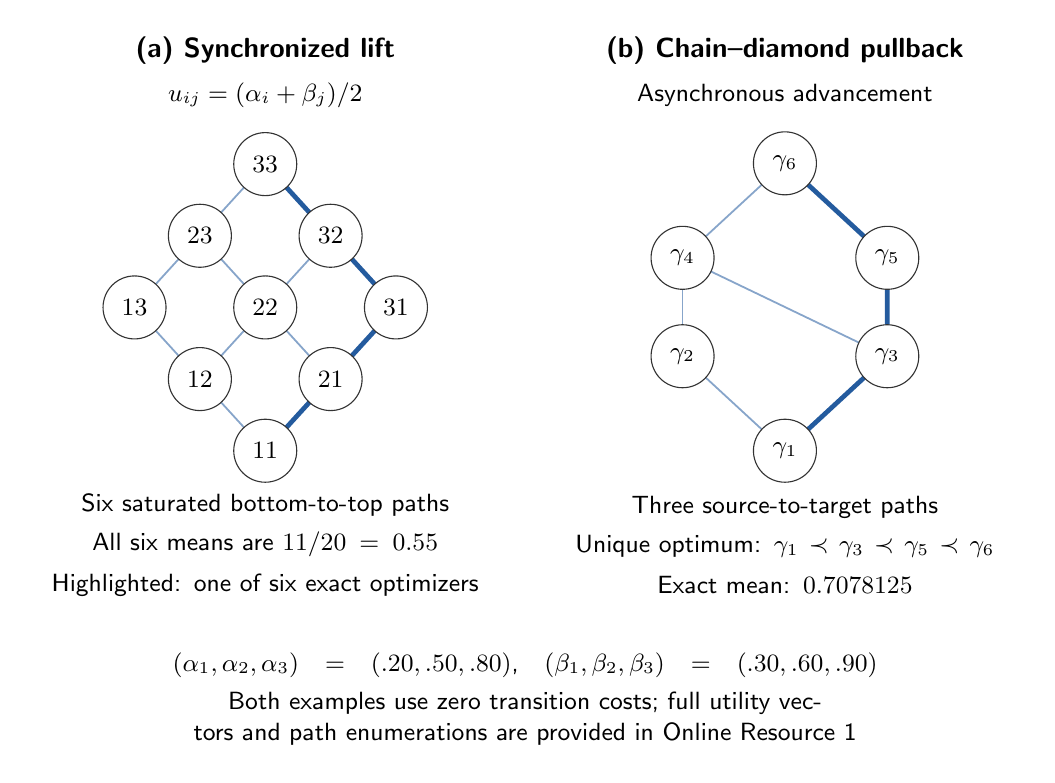
\begin{tikzpicture}[x=1cm,y=1cm]
\node[heading] at (0,5.28) {(a) Synchronized lift};
\node at (0,4.72) {$u_{ij}=(\alpha_i+\beta_j)/2$};
\coordinate (ip11) at (0.000,0.200);
\coordinate (ip12) at (-0.830,1.110);
\coordinate (ip13) at (-1.660,2.020);
\coordinate (ip21) at (0.830,1.110);
\coordinate (ip22) at (0.000,2.020);
\coordinate (ip23) at (-0.830,2.930);
\coordinate (ip31) at (1.660,2.020);
\coordinate (ip32) at (0.830,2.930);
\coordinate (ip33) at (0.000,3.840);
\draw[edge] (ip11) -- (ip21);
\draw[edge] (ip11) -- (ip12);
\draw[edge] (ip12) -- (ip22);
\draw[edge] (ip12) -- (ip13);
\draw[edge] (ip13) -- (ip23);
\draw[edge] (ip21) -- (ip31);
\draw[edge] (ip21) -- (ip22);
\draw[edge] (ip22) -- (ip32);
\draw[edge] (ip22) -- (ip23);
\draw[edge] (ip23) -- (ip33);
\draw[edge] (ip31) -- (ip32);
\draw[edge] (ip32) -- (ip33);
\draw[highlight] (ip11)--(ip21)--(ip31)--(ip32)--(ip33);
\node[vertex,minimum size=8mm] (i11) at (ip11) {$11$};
\node[vertex,minimum size=8mm] (i12) at (ip12) {$12$};
\node[vertex,minimum size=8mm] (i13) at (ip13) {$13$};
\node[vertex,minimum size=8mm] (i21) at (ip21) {$21$};
\node[vertex,minimum size=8mm] (i22) at (ip22) {$22$};
\node[vertex,minimum size=8mm] (i23) at (ip23) {$23$};
\node[vertex,minimum size=8mm] (i31) at (ip31) {$31$};
\node[vertex,minimum size=8mm] (i32) at (ip32) {$32$};
\node[vertex,minimum size=8mm] (i33) at (ip33) {$33$};
\node[align=center,text width=5.5cm] at (0,-1.0) {Six saturated bottom-to-top paths\\[3pt]All six means are $11/20=0.55$\\[4pt]Highlighted: one of six exact optimizers};
\node[heading] at (6.6,5.28) {(b) Chain--diamond pullback};
\node at (6.6,4.72) {Asynchronous advancement};
\coordinate (p1) at (6.6,0.2);
\coordinate (p2) at (5.3,1.4);
\coordinate (p3) at (7.9,1.4);
\coordinate (p4) at (5.3,2.65);
\coordinate (p5) at (7.9,2.65);
\coordinate (p6) at (6.6,3.85);
\draw[edge] (p1)--(p2);
\draw[edge] (p1)--(p3);
\draw[edge] (p2)--(p4);
\draw[edge] (p3)--(p4);
\draw[edge] (p3)--(p5);
\draw[edge] (p4)--(p6);
\draw[edge] (p5)--(p6);
\draw[highlight] (p1)--(p3)--(p5)--(p6);
\node[vertex,minimum size=8mm] at (p1) {$\gamma_1$};
\node[vertex,minimum size=8mm] at (p2) {$\gamma_2$};
\node[vertex,minimum size=8mm] at (p3) {$\gamma_3$};
\node[vertex,minimum size=8mm] at (p4) {$\gamma_4$};
\node[vertex,minimum size=8mm] at (p5) {$\gamma_5$};
\node[vertex,minimum size=8mm] at (p6) {$\gamma_6$};
\node[align=center,text width=5.9cm] at (6.6,-1.0) {Three source-to-target paths\\[3pt]Unique optimum: $\gamma_1\prec\gamma_3\prec\gamma_5\prec\gamma_6$\\[4pt]Exact mean: $0.7078125$};
\node[align=center,text width=12.4cm] at (3.3,-2.95) {$(\alpha_1,\alpha_2,\alpha_3)=(.20,.50,.80)$,\quad$(\beta_1,\beta_2,\beta_3)=(.30,.60,.90)$\\[3pt]
Both examples use zero transition costs; full utility vectors and path enumerations are provided in Online Resource 1};
\end{tikzpicture}
\end{document}
